\documentclass[14pt]{extarticle}

\usepackage{fontspec}
\usepackage{polyglossia}
\usepackage[a4paper, % Согласно требованиям к ВКР
  lmargin=30mm, rmargin=15mm, tmargin=20mm, bmargin=20mm]{geometry}
\usepackage{multirow}


\setdefaultlanguage{russian}
\setotherlanguage{english}



% Согласно требованиям к ВКР
\defaultfontfeatures{Ligatures=TeX}

\setmainfont{Times New Roman}
\setmonofont{Courier New}
\setsansfont{Arial}

\newfontfamily\cyrillicfont{Times New Roman}
\newfontfamily\cyrillicfontsf{Arial}
\newfontfamily\cyrillicfonttt{Courier New}

\newfontfamily\englishfont{Times New Roman}
\newfontfamily\englishfontsf{Arial}
\newfontfamily\englishfonttt{Courier New}

\linespread{1.5}

\usepackage[backend=biber,
  bibencoding=utf8,
  sorting=none,
  style=gost-numeric,
  language=autobib,
  autolang=other,
  clearlang=true,
  defernumbers=true,
  sortcites=true,
  doi=true,
  isbn=true,
  ]{biblatex}
\bibliography{bibliography}

\usepackage[dvipsnames]{xcolor}
\usepackage[hidelinks,colorlinks=false,citecolor=Black,urlcolor=Black]{hyperref}
\usepackage{caption}
\renewcommand{\UrlFont}{\small\rmfamily\tt}


\renewcommand\thesection{\arabic{section}}

\usepackage{amsfonts}

\usepackage{tikz}
\usepackage{pgfplots}
\usepackage{wrapfig}

\usepackage{graphicx}
\graphicspath{ {./images/} }

\setcounter{secnumdepth}{4}
\setcounter{tocdepth}{4}

% style end

% \renewcommand*{\maketitle}{
% \begin{titlepage}
  % \begin{center}
  %   \linespread{1}
  %   \small
  %   Федеральное государственное автономное образовательное учреждение\break высшего образования\par
  %   <<Московский физико-технический институт \break (национальный исследовательский университет)>>\par
  %   Физтех-школа Прикладной Математики и Информатики\par
  %   Кафедра корпоративных информационных систем\par
  % \end{center}
% 
  % {
  %   \footnotesize
  %   {\bf Направление подготовки / специальность}: 01.03.02 Прикладная математика и информатика\newline
  %   {\bf Направленность (профиль) подготовки}: Прикладная математика и компьютерные науки
  % }
%
  % {
  %   \topskip0pt
  %   \vspace*{\fill}
  %   \begin{center}
  %     {\bf\Large Разработка инструмента тестирования
  %     \break для курса распределенных систем}\par
  %     (бакалаврская работа)
  %   \end{center}
  %   \vspace*{\fill}
  % }
%
  % \hfill
  % \begin{minipage}[t]{8cm}
  %   {\bf Студент: \newline}
  %   Поминов Денис Игоревич\newline
  %   \vspace{-3mm}
  %   \rule{8cm}{0.15mm}
  %   \centerline{\scriptsize\it (подпись студента)}\newline
%
    % {\bf Научный руководитель: \newline}
%     Липовский Роман Германович\newline
%     \vspace{-3mm}
%     \rule{8cm}{0.15mm}
%     \centerline{\scriptsize\it (подпись научного руководителя)}
%   \end{minipage}

%     \vspace*{\fill}
%     \begin{center}
%       Москва 2022
%     \end{center}
% \end{titlepage}
% }

\usepackage{amsthm}

\usepackage{amsmath}
\usepackage{algorithm}
\usepackage[noend]{algpseudocode}

\makeatletter
\def\BState{\State\hskip-\ALG@thistlm}
\makeatother

\theoremstyle{definition}
\newtheorem*{definition}{Определение}

\newtheorem{theorem}{Теорема}
\newtheorem{task}{Задача}
\newtheorem{statement}{Утверждение}
\newtheorem{algo}{Алгоритм}
\newtheorem{implication}[statement]{Следствие}
\newtheorem{lemma}{Лемма}
\newtheorem*{comment}{Комментарий}

\DeclareMathOperator{\diam}{diam}

\begin{document}
% \maketitle

\newpage
\setcounter{page}{2}

\vspace*{\fill}
\begin{abstract}
Работа посвящена разработке инструмента для эффективного запуска графов обработки данных на MapReduce кластерах. Итоговый компонент - executor для библиотеки описания pipeline-ов Roren, исполняющий код поверх кластера YT.
\end{abstract}
\vspace*{\fill}

\newpage
\tableofcontents
\newpage

\section{Введение}
\label{sec:intro}

На 3 курсе ФПМИ МФТИ проводится курс по распределенным системам. Также этот курс читается на 4 курсе ФКН ВШЭ и 2 курсе ШАД.

При прохождении курса студенты решают практические задачи: написание распределенных сервисов с помощью фреймворка курса whirl \cite{whirl}. Код студентов запускается внутри среды исполнения, которая является детерминированной симуляцией распределенной системы.

Таким образом, основными пользователями фреймворка являются студенты. Далее мы будем отождествлять два этих слова.

Имеется потребность в написании тестирующего инструмента для данного курса распределенных систем. На данный момент тестирование является перебором некоторого количества состояний распределенного сервиса. На некоторых видах задач требуется увеличить покрытие тестирования.

Интеграция фреймворка курса с какими-либо аналогами невозможна, так как фреймворк является самописной разработкой на С++.

\subsection{Постановка задачи}

Инструмент должен решать задачу тестирования распределенной системы, внутри которой исполняется код студента.

Распределенную систему мы представим в виде набора узлов, объединенных в общую сеть. Узлы могут коммуницировать друг с другом только с помощью отправки сообщений.

Сеть мы считаем асинхронной и недетерминированной – она может произвольно задерживать и переупорядочивать отправляемые узлами сообщения. Если система будет корректно работать в асинхронной сети, то и в реальной, частично синхронной сети тоже.

Внутри узла исполняются недетерминированные программы. Также узлы могут отказывать, то есть перезагружаться в произвольные моменты и/или навсегда отключаться.

Мы считаем, что набор узлов системы реализует некоторый распределенный сервис, с которым клиенты взаимодействуют через протокол RPC. 

Клиенты тоже являются узлами сети. 

Они посылают системе запросы и получают ответы, в результате возникает конкурентная история, состоящая из отрезков запросов (рис.~\ref{fig:history_example}). Свойства системы формулируются как утверждения про допустимые истории, которые может порождать система.

\begin{figure}[h]
    \centering
    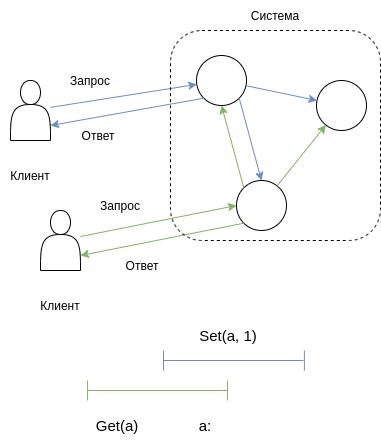
\includegraphics[width=0.5\textwidth]{img/task.png}
    \caption{Пример истории запросов}
    \label{fig:history_example}
\end{figure}

В данной работе нас прежде всего интересует задача репликации, так что распределенный сервис  представляет собой хранилище данных с операциями Set и Get, а свойство, которое мы ожидаем от системы – модель согласованности \cite{consistency}, в первую очередь – линеаризуемость \cite{linearizability}.

Наконец, сформулируем задачу – по реализации узлов системы проверить выполнение заявленных свойств независимо от поведения сети между узлами, часов и т.д.

\subsection{Цель работы}

Цель работы состоит в реализации части библиотеки Roren, отвечающей за перевод и выполнение pipeline-ов поверх YT. Компонент должен позволять запускать произвольные графы обработки данных, выражаемые операциями Map/Reduce.

Получившаяся реализация в сравнении с текущей должна:
\begin{itemize}
    \item Переводить pipeline-ы в графы с меньшим количеством YT операций
    \item Иметь расширяемый на более сложные YT операции алгоритм трансляции
\end{itemize}

\subsection{План работы}

Во второй главе мы рассмотрим дизайн библиотеки Roren: от API pipeline-ов до запуска YT операций.

В третьей главе рассмотрим реализацию компонента, производящего трансляцию. Мы изложим этапы перевода roren графа в граф YT операций, алгоритм трансляции, и детально остановимся на компоненте оптимизатора.

В четвертой главе посмотрим на примеры графов и их трансляций, обсудим тестирование.

В последней главе мы поговорим о результатах работы и обсудим пути развития компонента.


\section{Дизайн библиотеки Roren}
\label{sec:design}

Дизайн библиотеки Roren построен аналогично open-source инструменту Apache Beam \cite{beam}.

Apache Beam предлагает универсальный API для создания сложных pipeline-ов обработки данных, которые можно запускать на различных движках. В случае Roren движки называют executor-ами. Основные принципы этого уровня основаны на модели Beam (ранее известной как модель Dataflow \cite{dataflow}) и реализованы в различной степени в каждом из executor-ов Roren.

Такой дизайн позволяет разработчикам проектировать масштабируемые приложения для обработки данных, которые могут адаптироваться к разным технологическим платформам и инфраструктурам без необходимости изменения кода. Использование Roren упрощает интеграцию с различными источниками данных и позволяет эффективно управлять потоками данных и их обработкой в реальном времени.

\newpage
\subsection{Interface graph}

Библиотека Roren включает в себя несколько абстракций, которые упрощают процесс обработки данных в условиях больших распределенных систем. Эти абстракции применимы как к batch, так и к streaming источникам данных. При создании pipeline-а есть возможность структурировать задачи обработки данных, используя абстракции преобразований данных и результатов их применений - transform-ов и collection-ов соответственно.

Pipeline описывает всю задачу обработки данных от начала до конца. Он включает в себя чтение входных данных, их преобразование и запись выходных таблиц. При его создании есть возможность указать параметры выполнения, специфичные для конкретного паттерна выполнения: настройки streaming или MapReduce инфраструктуры.

Collection представляет собой распределенный набор данных, с которым работает pipeline. Набор данных может быть ограниченным, то есть происходить из фиксированного источника, как файл, или неограниченным, то есть поступать из постоянно обновляющегося streaming источника. Типичный pipeline создает начальный collection, читая данные из внешнего источника данных. Далее, коллекции служат входными и выходными данными для каждого преобразования в pipeline.

Transform представляет операцию обработки данных. Каждый transform принимает один или несколько объектов collection в качестве входных данных, выполняет функцию обработки, которую пользователь предоставляет, над элементами этой коллекции данных, а затем производит ноль (в случае стока графа - записи во внешнее хранилище) или более выходных объектов collection.

Roren включает множество I/O преобразований - библиотечных transforms, которые читают или записывают данные в различные внешние системы хранения данных. Чтения и записи таблиц в случае MapReduce или топиков брокеров сообщений осуществляются через общие интерфейсы IRawRead и IRawWrite.

Трансформации могут изменять, фильтровать, группировать, анализировать или иным образом обрабатывать элементы collection-а. Преобразование создает новую выходную коллекцию данных, не модифицируя входную коллекцию. Типичный pipeline применяет последующие трансформации к каждой новой выходной collection по очереди, пока обработка не будет завершена. Однако стоит отметить, что пайплайн не обязательно должен быть одной прямой линией трансформаций, применяемых одна за другой. Можно рассматривать коллекции как переменные, а преобразования как функции, применяемые к этим переменным, что позволяет создать сложный граф обработки.

После того, как в коде описаны все transform-ы, pipeline запускается с использованием назначенного executor-а (рис~\ref{fig:pipeline}).

\begin{figure}[h]
    \centering
    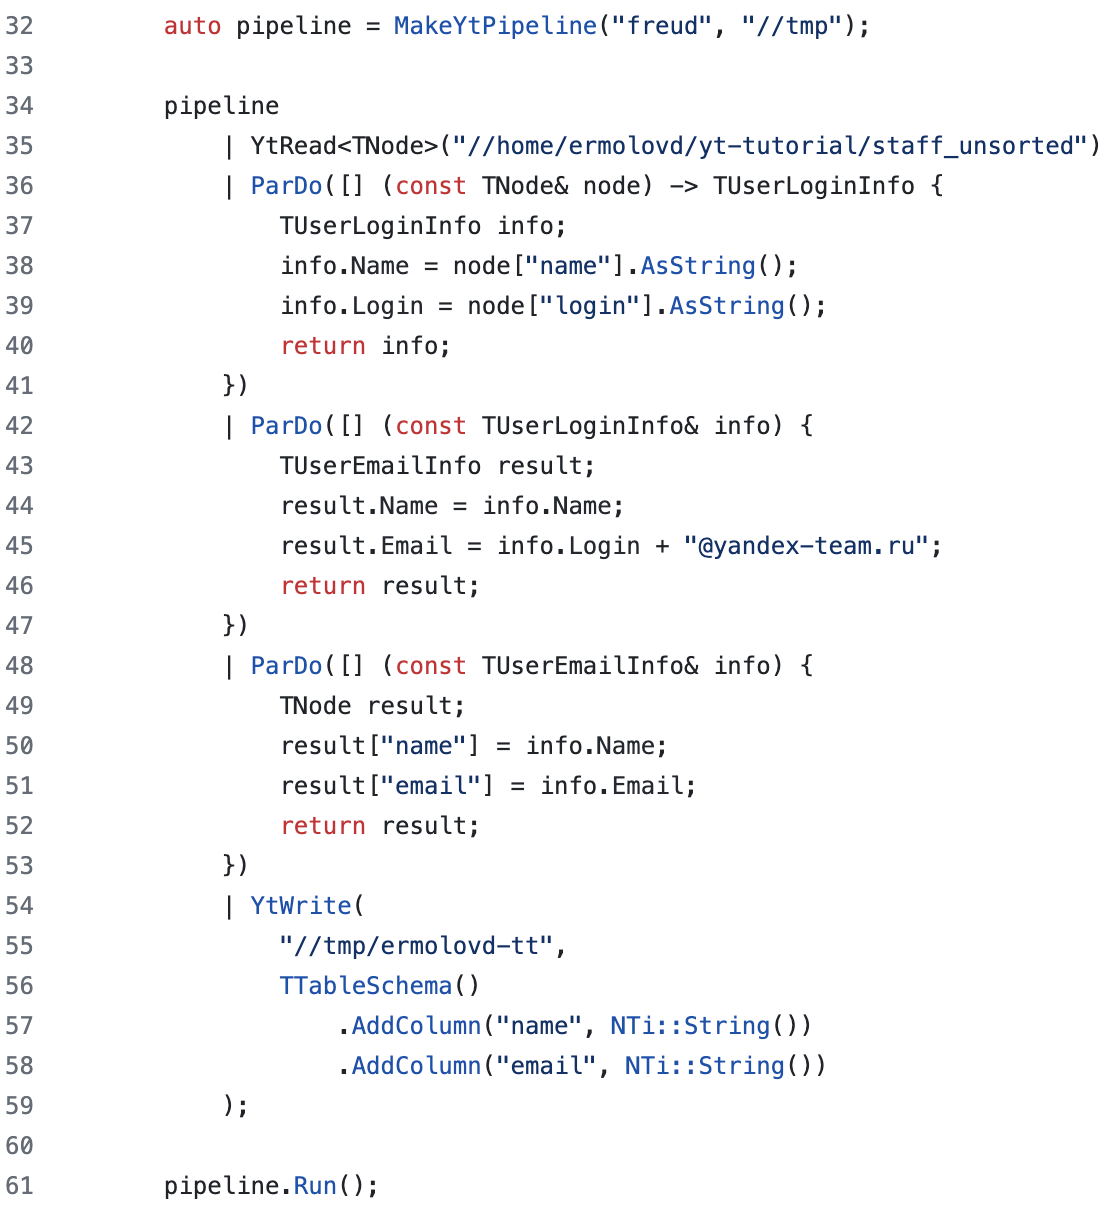
\includegraphics[width=\textwidth]{img/pipeline.png}
    \caption{Типичный pipeline с YT executor-ом}
    \label{fig:pipeline}
\end{figure}

\newpage
\subsection{Понятие executor-а}

Executor - это движок, отвечающий за то, каким именно образом данные поступают и обрабатываются графом transform-ов.

В простейшем случае streaming процессинга пользователь указывает входные топики брокера логов или очереди сообщений, ожидая, что данные относительно небольшими порциями будут вычитаны из источников, к ним применяются transform-ы и они будут записаны в выходные топики, очереди или таблицы.

В случае batch процессинга после указания входных и выходных таблиц с помощью примитивов API pipeline-а ожидается запуск некоторого количества операций, а как следствие Map/Reduce job-ов на кластере. Вместе эти операции будут эквивалентны применению к входным данным преобразований, указанных пользователем.

На этом этапе можно задуматься, что ParDo соответствует Map операции запущенной на кластере, а GroupByKey - Reduce.

\newpage
\subsection{YT executor}

Далее мы рассмотрим специфику запуска именно на YT Map/Reduce кластере.

Api YT имеет возможность создания операций с многими входами, многими выходами. Причем зачастую, есть возможность писать выходные таблицы с промежуточных стадий составных операций.

Если рассмотреть некоторый подграф, состоящий целиком из ParDo, то теоретически ничто не мешает запустить его как одну Map операцию, которая внутри себя сохраняет структуру вызова пользовательских функций из ParDo. Наличие возможности указать многие входы и выходы операции позволяет запускать подграфы с несколькими истоками и стоками.

В свою очередь, GroupByKey в общем случае может быть представлен в виде MapReduce операции. Это объясняется тем, что перед функцией группировки будут вызвано какое-то количество ParDo преобразующих входные данные из YSON \cite{yson} формата во внутреннее представление пары ключ-значение.

Существует важное замечание, что MapReduce - это операция Map, решардирование с помощью хэширования и запуск Reduce. Такого рода операция эффективнее Map, сортировки данных и Reduce.

I/O общение с таблицами кластера осуществляется через реализацию RawRead и RawWrite - YtRead и YtWrite. C помощью YtRead можно чтения таблиц в YSON или Protobuf \cite{protobuf} форматах. YtWrite имеет возможность указания схемы, в том числе сортированной, для записи выходных значений. Так как рассматриваемая в данной работе реализация является proof-of-concept, мы опускаем реализации I/O в формате Protobuf и сортированных данных.


\section{Реализация executor-a}
\label{sec:executor}

Был реализован отдельный drop-in executor с несколькими этапами трансляции.

На первом этапе из pipeline и сущностей API собирается граф, который содержит похожие на roren transform-ы вершины. Разница здесь в том, что это отдельные примитивы, которые легко сливаются. Так же в графе существуют collection-ы, напрямую взятые из графа API.

Далее следует стадии оптимизации, которая может быть тривиальной. Ниже по тексту рассмотрим именно такой случай, а позже поставим оптимизатор на свой этап.

Завершающим этапом является перевод в граф YT операций.

\newpage
\subsection{Построение Roren graph-a}

Отдельная вершина, в которую происходит трансляция roren transform-ов - это wrapper или обертка. Рассматриваемая обертка должна хранить в себе информацию о положении в исходном графе, тип transform-а, входные и выходные collection-ы.

Из wrapper-ов построена иерархия. Существует единый интерфейс обертки, который частично реализуют гранулярный wrapper и графовый wrapper [картинка]. Логически гранулярный wrapper - это набор некоторых Part-ов, которые в себе сохраняют информацию о преобразовании, его входных и выходных коллекциях. В свою очередь, графовый wrapper хранит уникальный идентификатор вершины и глубину слоя в графе [картинка].

Далее по иерархии в соответствие с transform-ами из API Roren сопоставлены wrapper: ReadWrapper, WriteWrapper, ParDoWrapper, GroupByKeyWrapper и FlattenWrapper.

У ParDoWrapper-а есть возможность сколлапсировать с другим ParDoWrapper-ом. Это естественная возможность, т.к. логически ParDo является фукнцией над некоторыми входными данными, а коллапсирование - способ выразить композицию функций. Однако помимо объединения в композицию функций из двух функций с разными входами можно сделать одну с многими входными таблицами.

Здесь важно заметить, что практически каждый wrapper может иметь входные или выходные таблицы, кроме GroupByKeyWrapper и FlattenWrapper. Очевидно, что ReadWrapper и WriteWrapper имеют какие-то входные и выходные таблицы соответственно. Ради упрощения конденсации графа, ParDo Wrapper в отличие от ParDo может иметь входные и выходные таблицы, как результат слияния с ReadWrapper или WriteWrapper.

\newpage
\subsection{Трансляция в граф YT операций}

Отдельный компонент отвечает за перевод RorenGraph-а в граф YT операций. Это включает в себя преобразование узлов, отвечающих за фильтрацию, агрегацию и трансформацию данных, в задачи Map и Reduce в YT. Основной вызов здесь — обеспечить, чтобы все зависимости и последовательности операций были правильно интерпретированы и перенесены, сохраняя при этом оптимальную производительность и масштабируемость в новой среде.

Граф из полученных операций может быть запущенной под общей транзакцией. Операции будут запущены с учетом причинности, конкретнее в топологическом порядке по слоям.

На этом этапе сложность составляет сопоставление входных и выходных таблиц файловым дескрипторам, через которые происходит запись в YT job. Помимо этого, информация о конденсированных подграфах должна быть сериализуема для запуска в виде job-a на Map/Reduce кластере.

\newpage
\subsection{Алгоритм оптимизации}

\input{parts/executor/algo/00}
\newpage
\input{parts/executor/algo/01}


\newpage
\subsection{Оптимизатор}

Стадия оптимизации подразумевает несколько обходов по заранее построенному RorenGraph-у.

\subsubsection{Стратегии оптимизации}

В оптимизаторе отдельно выделен интерфейс IStrategy (рис~\ref{fig:strat}), позволяющий коллапсировать оранжевую и красную вершину связанные ребром. Важно, что этот случай подразумевает, что нет другой оранжевой вершины, ребра которой ведут в рассматриваемую красную.

\begin{figure}[h]
    \centering
    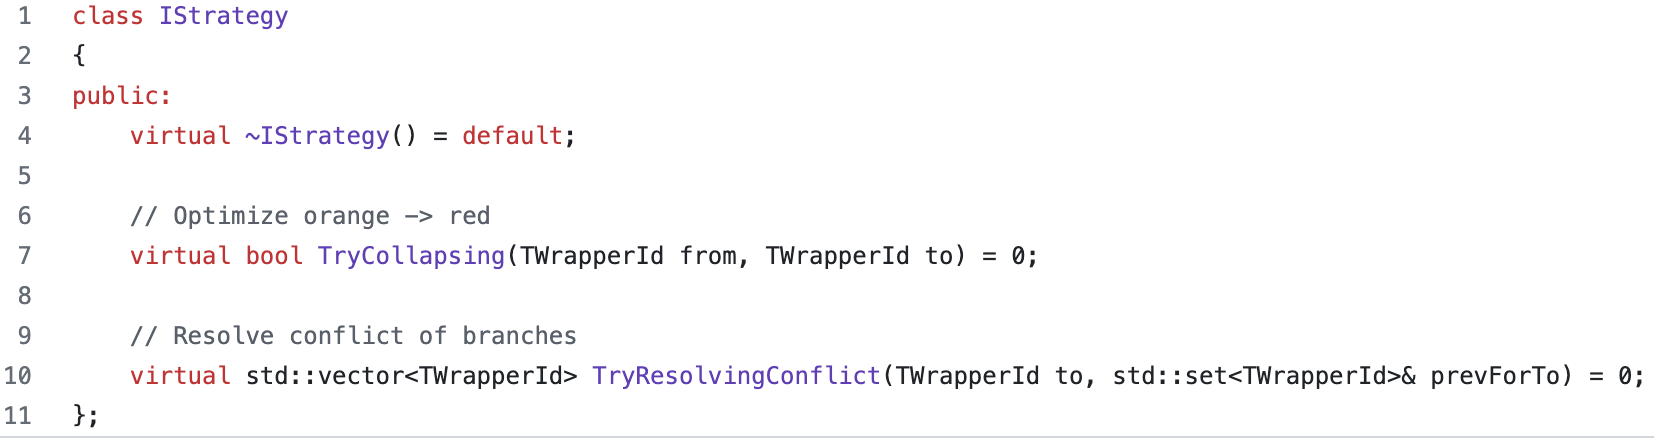
\includegraphics[width=\textwidth]{img/strat.png}
    \caption{Интерфейс стратегии конденсации вершин}
    \label{fig:strat}
\end{figure}

Помимо этого IStrategy позволяет разрешить конфликтную ситуацию, когда есть множество оранжевых вершин, ребра которых ведут в общую красную вершину.

Реализацией данной стратегии может быть стратегия, которая коллапсирует вершины и разрешает конфликты.

Однако это далеко не единственный вариант. Пользователям может понадобится стратегия, которая не сливает параллельные ветви, т.к. это увеличивает latency готовности конкретных таблиц.

Также пользователи могут иметь вычислительно тяжелые операции, требующие большого количества RAM. Так, в случае отдельного запуска операций проблем не будет, но при их слиянии памяти, отведенной на один job, может не хватить.

\newpage
\subsubsection{Предобход для Flatten}

В дизайн Roren заложена концепция, которая позволяет легко описывать в коде графы. Она состоит в том, что у transform-а может быть только один вход. В случае графов с Flatten такой дизайн приведет к тому, что требуется рассматривать несколько слоев transform-ов. Также для упрощения алгоритма мы рассматриваем граф, состоящий из transform-ов, не обращая внимания на коллекции, но сохраняя их.

Для того, чтобы перейти к упрощенному графу требуется сделать предобход, который удалить из графа Flatten, соединяя предыдущие и последующие transform-ы напрямую.

\newpage
\subsection{Дополнения алгоритма}

\subsubsection{Сохранение сортированности}

\newpage
\subsubsection{Когда не стоит оптимизировать}


\section{Запуск pipeline-ов}
\label{sec:pipeline}

\subsection{Уровни оптимизации}

Для проверки корректности каждого из этапов оптимизации удобно не писать дополнительные тесты, а отключать некоторые из этапов, проверяя, что корректность итогового графа не ломается. Например, можно не делать предобход Flatten, если представить Flatten - как тривиальный ParDo. В свою очередь как YT операция Flatten представляется в виде тривиального Map-a.

Есть возможность отключать полностью любые оптимизации, проверяя, находится ли ошибка в коде построение RorenGraph-а или вне него.

\newpage
\subsection{Анализ исполнений}

На картинках приведены примеры исходных API графов, полученных из них графов операций YT [картинка].


\section{Заключение}
\label{sec:conclusion}

\subsection{Результаты}

Реализован инструмент – model checker, интегрированный в фреймворк курса whirl \cite{checkers}.

Model checker способен проверять инварианты пользовательского кода во время обхода графа конфигураций. При нахождении исполнения нарушающего пользовательский предикат, инструмент выводит детализированный лог.  В написанном model checker-е есть возможность тестирования детерминизма.

Реализация инструмента протестирована на содержательном примере: сервис, реализующий атомарный регистр с помощью алгоритма ABD. Пользовательский код можно писать пользуясь всеми средствами выразительности фреймворка whirl.

Инструмент отрабатывает перебор состояний на нетривиальных примерах за разумное время. При валидации укладывается в лимиты по памяти.


\newpage
\subsection{Планы на будущее}

Задача написания инструмента подобного рода не решается идеально. Основное фундаментальное ограничение – экспоненциальный рост числа состояний с ростом числа сообщений в системе. Существует несколько аспектов, которые можно доработать:

\begin{itemize}
    \item Ускорение алгоритма перебора за счет отсечения симметричных ветвей \cite{dpor}.
    \item Поддержка таймеров. Это возможно сделать через отправку узлом специального сообщения себе.
    \item Визуализация исполнения с нарушением инварианта в виде графа доставки сообщений.
\end{itemize}



\newpage
\printbibliography
\end{document}
